%% =====================================================================
%% Báo cáo kỹ thuật -- Kỹ thuật Dữ liệu (CO5173), HCMUT -- Nhóm 27
%% Kho dữ liệu mô hình chiều Kimball cho phân tích dòng tiền ngân hàng (Berka)
%% Bản tiếng Việt của main.tex (nội dung giữ nguyên, chỉ dịch).
%%
%% Định dạng và cấu trúc theo mẫu báo cáo kỹ thuật IEEE trong
%% LaTeX_Template_for_Technical_Report/ (IEEEtran v1.8, peerreview).
%% IEEEtran.cls phải nằm cạnh tệp này.
%% Biên dịch: tectonic main_vi.tex   (hoặc XeLaTeX trên Overleaf, chạy hai lần)
%% Tệp này cần XeLaTeX (fontspec + polyglossia); không biên dịch bằng pdfLaTeX.
%% Các mục [TODO] màu đỏ là các quyết định còn chờ nhóm thống nhất.
%% =====================================================================

\documentclass[peerreview]{IEEEtran}
\usepackage{cite}      % Tidies up citation numbers.
\usepackage{url}       % Provides better formatting of URLs.
\usepackage{fontspec}
% TeX Gyre Termes / Cursor (cover Vietnamese). Loaded by file name so that the
% fonts are found both by tectonic and by XeLaTeX on Overleaf.
\setmainfont{texgyretermes}[Extension=.otf, UprightFont=*-regular,
  BoldFont=*-bold, ItalicFont=*-italic, BoldItalicFont=*-bolditalic]
\setmonofont{texgyrecursor}[Extension=.otf, UprightFont=*-regular,
  BoldFont=*-bold, ItalicFont=*-italic, BoldItalicFont=*-bolditalic]
\usepackage{polyglossia}
\setdefaultlanguage{vietnamese}
\usepackage{booktabs}  % \toprule, \midrule and \bottomrule in tables
\usepackage{graphicx}
\graphicspath{{figures/}}

% ---------- Additional packages ----------
\usepackage{amsmath,amssymb}
\usepackage{array}
\usepackage{xcolor}
\usepackage{listings}
\usepackage{tikz}
\usetikzlibrary{arrows.meta,positioning,fit}
\usepackage[hidelinks]{hyperref}

% ---------- Float placement ----------
% Allow a few more floats per page; create a float-only page only when
% it would be nearly full.
\setcounter{topnumber}{3}
\setcounter{bottomnumber}{2}
\setcounter{totalnumber}{5}
\setcounter{dbltopnumber}{2}
\renewcommand{\topfraction}{0.85}
\renewcommand{\bottomfraction}{0.6}
\renewcommand{\textfraction}{0.1}
\renewcommand{\floatpagefraction}{0.85}
\renewcommand{\dbltopfraction}{0.85}
\renewcommand{\dblfloatpagefraction}{0.85}

\hyphenation{op-tical net-works semi-conduc-tor}

% ---------- Helpers ----------
\newcommand{\todo}[1]{\textcolor{red}{[TODO: #1]}}
\newcommand{\tbl}[1]{\texttt{#1}}
\newcolumntype{L}[1]{>{\raggedright\arraybackslash}p{#1}}

\lstdefinestyle{code}{
  basicstyle=\ttfamily\scriptsize,
  keywordstyle=\color{blue!70!black}\bfseries,
  commentstyle=\color{green!40!black}\itshape,
  stringstyle=\color{orange!70!black},
  breaklines=true,
  frame=single,
  framesep=3pt,
  columns=fullflexible,
  keepspaces=true,
  showstringspaces=false,
  captionpos=b
}
\lstset{style=code}


\begin{document}

% Vietnamese names for floats and lists (set after \begin{document} so that
% IEEEtran and polyglossia do not override them).
\renewcommand{\tablename}{Bảng}
\renewcommand{\figurename}{Hình}
\renewcommand{\lstlistingname}{Mã nguồn}
\renewcommand{\contentsname}{Mục lục}
\renewcommand{\listfigurename}{Danh sách hình}
\renewcommand{\listtablename}{Danh sách bảng}
\renewcommand{\abstractname}{Tóm tắt}
\renewcommand{\refname}{Tài liệu tham khảo}
\renewcommand{\appendixname}{Phụ lục}

% paper title
\title{Kho dữ liệu mô hình chiều Kimball cho phân tích dòng tiền ngân hàng: \\
Thiết kế, triển khai và đánh giá \\ với Spark, ClickHouse và PostgreSQL}

% author names and affiliations
\author{Kiet Ho Tuan Nguyen, Quan Minh Tran, Van Ngoc Huynh, Hai Ngoc Ho \\
Nhóm 27 --- Kỹ thuật Dữ liệu (CO5173), Học kỳ 1, 2026--2027\\
Khoa Khoa học và Kỹ thuật Máy tính\\
Trường Đại học Bách khoa (HCMUT), ĐHQG-HCM\\
Giảng viên: Assoc. Prof. Dr. Chau Thi Ngoc Vo\\
}
\date{\todo{ngày nộp}}

% make the title area
\maketitle
\tableofcontents
\listoffigures
\listoftables

\IEEEpeerreviewmaketitle

\begin{abstract}
Một ngân hàng cần câu trả lời đáng tin cậy về cách tiền lưu chuyển, về những gì đã xảy ra
trên một tài khoản, và về việc dữ liệu đứng sau các câu trả lời đó có đáng tin cậy hay
không. Chúng tôi xây dựng và đánh giá một giải pháp kỹ thuật dữ liệu cho các nhu cầu này
trên bộ dữ liệu Berka của một ngân hàng Séc (1.056.320 giao dịch, 1993--1998), được bổ sung
một hạng thành viên mô phỏng mà lịch sử của nó phải được lưu giữ. Giải pháp là một kho dữ
liệu Kimball---một bảng fact giao dịch và năm dimension, trong đó có một dimension khách hàng
Type~2---được nạp theo lô bằng Apache Spark qua một Data Lake dạng Parquet vào ClickHouse,
cùng một kho dữ liệu vận hành trên PostgreSQL cho các lần chạy, bản ghi bị tách, cảnh báo
gian lận và sao lưu, và một ứng dụng Streamlit duy nhất phục vụ ba nhóm người dùng và tám
yêu cầu nghiệp vụ. Tám kịch bản đánh giá, mỗi kịch bản đều được đối soát với nguồn, đạt cả
38 phép kiểm tra, và tổng dòng tiền khớp với nguồn đến từng xu. Bốn benchmark, mỗi benchmark
chỉ thay đổi một yếu tố, cho thấy ClickHouse trả lời các truy vấn tổng hợp nhanh hơn
3,3--22 lần so với cùng star schema trên PostgreSQL (7--28 lần trên một bản sao nhân mười
lần) với dung lượng nhỏ hơn 8,7 lần; One Big Table chỉ tiết kiệm được vài mili giây nhưng
phải ghi lại 150.058 dòng để sửa một khu vực; và kho vận hành nhanh hơn 8--70 lần trong
PostgreSQL, vốn còn thực thi các quy tắc toàn vẹn mà ClickHouse không thực thi. Mọi yêu cầu
đều được trả lời với một đến ba thao tác.
\end{abstract}


%% =====================================================================
\section{Giới thiệu}
\label{sec:intro}

Mỗi lần gửi tiền, thanh toán hay rút tiền của một ngân hàng đều để lại một bản ghi. Khi được
tổng hợp, các bản ghi này cho thấy tiền lưu chuyển qua ngân hàng như thế nào và từng tài
khoản hoạt động ra sao---nhưng nhật ký giao dịch thô không trả lời trực tiếp được các câu hỏi
đó: mã của chúng ngắn gọn và thiếu một phần, thuộc tính của khách hàng thay đổi mà không lưu
lại lịch sử, và không có gì trong đó cho người dùng biết lần nạp gần nhất có thành công
không hay một báo cáo trước đây có còn đúng hay không.

Báo cáo này trình bày đề tài của Nhóm~27 thuộc môn Kỹ thuật Dữ liệu (CO5173). Lĩnh vực ứng
dụng là \textbf{ngân hàng} và giải pháp là một \textbf{kho dữ liệu mô hình chiều theo
Kimball} \cite{kimball2013}. Mục tiêu là chứng minh, bằng căn cứ đo lường được, rằng giải
pháp biến các giao dịch ngân hàng thô thành dữ liệu đúng, truy vấn nhanh và hữu ích cho
người dùng của ngân hàng. Các đóng góp chính gồm:
\begin{itemize}
  \item một star schema (lược đồ hình sao) với một dimension (bảng chiều) khách hàng Type~2
        lưu giữ lịch sử của một hạng thành viên;
  \item một pipeline theo lô tách riêng các bản ghi lỗi, chạy lại mà không tạo bản trùng, và
        ghi lại mọi lần chạy vào một kho vận hành, được điều khiển từ một ứng dụng;
  \item một đánh giá qua tám kịch bản được đối soát với nguồn và bốn benchmark so với các
        giải pháp thay thế.
\end{itemize}
Mục~\ref{sec:problem} định nghĩa bài toán, Mục~\ref{sec:solutions} trình bày các giải pháp,
Mục~\ref{sec:criteria} các tiêu chí đánh giá, Mục~\ref{sec:method} phương pháp nghiên cứu,
Mục~\ref{sec:analysis} các kết quả, và Mục~\ref{sec:conclusion} kết luận.


%% =====================================================================
\section{Định nghĩa bài toán}
\label{sec:problem}

\subsection{Phát biểu bài toán}
\begin{quote}
\emph{Làm thế nào để xử lý dữ liệu giao dịch của một ngân hàng thành một kho dữ liệu đúng,
hiệu năng cao và khai thác được, với các lần nạp được kiểm soát, lịch sử được lưu giữ, và có
thể chứng minh là đáp ứng các yêu cầu nghiệp vụ của nhiều nhóm người dùng?}
\end{quote}

\subsection{Nhóm người dùng và yêu cầu nghiệp vụ}
Nhóm đã xác định ba nhóm người dùng, mỗi nhóm được phục vụ bởi một tab của ứng dụng
(Bảng~\ref{tab:usergroups}). Với bốn thành viên, môn học yêu cầu tối thiểu tám yêu cầu
nghiệp vụ (BR); mỗi BR đi kèm một kịch bản đánh giá (KB01--KB08) có kết quả mong đợi được
viết trước khi nạp dữ liệu (Bảng~\ref{tab:brs}). Các BR cùng phục vụ bốn mục tiêu: theo dõi
dòng tiền (BR01, BR08), phục vụ tra cứu tài khoản (BR02), giảm tổn thất do gian lận (BR03,
BR04), và bảo đảm dữ liệu và vận hành đáng tin cậy (BR05--BR07).

\begin{table}[!t]
\centering
\caption{Các nhóm người dùng}
\label{tab:usergroups}
\footnotesize
\setlength{\tabcolsep}{4pt}
\begin{tabular}{L{2.0cm} L{3.3cm} L{2.4cm}}
\toprule
\textbf{Nhóm người dùng} & \textbf{Nhu cầu} & \textbf{Tab / BR} \\
\midrule
U01 Quản lý kinh doanh & Tổng quan dòng tiền và lịch sử theo hạng & Tổng quan / BR01 \\
U02 Chuyên viên phân tích & Tra cứu tài khoản; xem xét và xử lý cảnh báo & Phân tích / BR02--BR04 \\
U03 Kỹ sư dữ liệu & Chất lượng dữ liệu, pipeline, sao lưu, lịch sử & Vận hành / BR05--BR08 \\
\bottomrule
\end{tabular}
\end{table}

\begin{table*}[!t]
\centering
\caption{Yêu cầu nghiệp vụ và kịch bản đánh giá}
\label{tab:brs}
\small
\begin{tabular}{l l L{6.6cm} L{6.4cm}}
\toprule
\textbf{Mã} & \textbf{Người dùng} & \textbf{Yêu cầu nghiệp vụ} & \textbf{Kịch bản đánh giá (kết quả mong đợi)} \\
\midrule
BR01 & U01 & Tổng quan dòng tiền: tiền vào, tiền ra, dòng tiền thuần và số giao dịch trong một kỳ, theo hạng, dưới dạng biểu đồ theo ngày hoặc theo tháng & KB01: số liệu bằng kết quả một truy vấn trên nguồn \\
BR02 & U02 & Hoạt động tài khoản: các giao dịch và các tổng của một tài khoản trong một kỳ & KB02: các giao dịch bằng nguồn, từng giao dịch một \\
BR03 & U02 & Phát hiện gian lận: sau mỗi lần nạp, sinh cảnh báo kèm lý do và căn cứ & KB03: một lô gian lận được chuẩn bị sẵn sinh ra đúng các cảnh báo mong đợi \\
BR04 & U02 & Xử lý cảnh báo: \emph{chưa xem / đang xem xét / đã xử lý}, kèm ghi chú và lịch sử & KB04: thay đổi trạng thái được ghi lại và hiển thị trên giao diện \\
BR05 & U03 & Kiểm soát dữ liệu: kiểm tra từng lô, tách riêng bản ghi không đạt kèm lý do & KB05: một lô chứa lỗi cố ý được tách đúng \\
BR06 & U03 & Giám sát pipeline: các bước, trạng thái, thời điểm, số lượng, nguyên nhân lỗi & KB06: xác định được bước lỗi và nguyên nhân \\
BR07 & U03 & Sao lưu và khôi phục sáu bảng của kho dữ liệu, kể cả lịch sử SCD & KB07: sau khi khôi phục, số liệu bằng bản sao lưu \\
BR08 & U03 & Báo cáo lịch sử: việc đổi hạng không được làm thay đổi báo cáo của các kỳ trước (SCD2) & KB08: kỳ cũ không đổi, kỳ mới theo hạng mới \\
\bottomrule
\end{tabular}
\end{table*}

\subsection{Nguồn dữ liệu}
\label{sec:data-source}
Bộ dữ liệu Berka \cite{berka1999} chứa các bản ghi đã ẩn danh của một ngân hàng Séc. Mỗi tệp
Berka đại diện cho một hệ thống của ngân hàng (Bảng~\ref{tab:sources}); khoản vay, lệnh chi
định kỳ và thẻ nằm ngoài phạm vi của các BR. Số giao dịch trong 1.056.320 giao dịch tăng từ
28.205 năm 1993 lên 322.277 năm 1998, và mỗi tài khoản có từ 9 đến 675 giao dịch (trung vị
208). Mỗi tài khoản có đúng một chủ sở hữu, và 409 tài khoản thuộc một khu vực chi nhánh
khác với khu vực cư trú của chủ sở hữu, vì vậy khu vực đóng hai vai trò. Mã \tbl{type} cho
biết chiều của dòng tiền (Bảng~\ref{tab:types}); số tiền không bao giờ âm. Việc khảo sát
dữ liệu (profiling) tái hiện được 14 trên 15 số liệu trong khảo sát trước đó của nhóm về bộ
dữ liệu.

\begin{table}[!t]
\centering
\caption{Các tệp nguồn}
\label{tab:sources}
\footnotesize
\setlength{\tabcolsep}{4pt}
\begin{tabular}{L{2.75cm} L{3.15cm} r}
\toprule
\textbf{Tệp} & \textbf{Đại diện cho} & \textbf{Số dòng} \\
\midrule
\tbl{trans} & Hệ thống ngân hàng lõi & 1.056.320 \\
\tbl{account} & Sổ đăng ký tài khoản & 4.500 \\
\tbl{client}, \tbl{disp} & Dữ liệu gốc khách hàng (chủ sở hữu) & 5.369 \\
\tbl{district} & Dữ liệu tham chiếu (77 khu vực) & 77 \\
\tbl{customer\_profile\_\allowbreak simulated} & Hệ thống khách hàng thân thiết (hạng mô phỏng) & 4.500 \\
\bottomrule
\end{tabular}
\end{table}

\begin{table}[!t]
\centering
\caption{Loại giao dịch và chiều dòng tiền (số tiền tính bằng CZK)}
\label{tab:types}
\footnotesize
\setlength{\tabcolsep}{2.5pt}
\begin{tabular}{l l r r r r}
\toprule
\textbf{Loại} & \textbf{Chiều} & \textbf{Số lượng} & \textbf{Tỷ lệ} & \textbf{Trung vị} & \textbf{Tổng (tr.)} \\
\midrule
VYDAJ (ghi nợ) & OUT & 634.571 & 60,07\% & 2.042 & 2.821,7 \\
PRIJEM (ghi có) & IN & 405.083 & 38,35\% & 1.600 & 3.227,5 \\
VYBER (rút tiền) & OUT & 16.666 & 1,58\% & 12.103 & 208,6 \\
\bottomrule
\end{tabular}
\end{table}

\subsection{Khiếm khuyết chất lượng dữ liệu}
\label{sec:data-quality}
Các khiếm khuyết liên quan đến việc phân loại giao dịch chứ không phải số tiền
(Bảng~\ref{tab:dq}, theo ISO/IEC 25012 \cite{iso25012}).

\begin{table*}[!t]
\centering
\caption{Khiếm khuyết chất lượng dữ liệu theo đặc tính ISO/IEC 25012}
\label{tab:dq}
\small
\begin{tabular}{L{2.3cm} L{7.0cm} L{5.4cm}}
\toprule
\textbf{Đặc tính} & \textbf{Phát hiện} & \textbf{Cách xử lý} \\
\midrule
Tính đầy đủ & \tbl{operation} rỗng ở 183.114 giao dịch; \tbl{k\_symbol} là NULL ở 481.881 và rỗng ở 53.433 giao dịch & Thành viên tường minh \texttt{NOT\_RECORDED}; không bỏ dòng nào \\
Tính nhất quán & Hai cách mã hóa giá trị ``thiếu''; mã bị chèn khoảng trắng; 17 tổ hợp nhưng chỉ mang 15 nghĩa & Chuẩn hóa thành một junk dimension gồm 15 hồ sơ \\
Tính dễ hiểu & Mã tiếng Séc (ví dụ \texttt{PRIJEM}, \texttt{SIPO}) & Tên dễ đọc và chiều dòng tiền \\
Tính chính xác & Ngày sinh và giới tính được gộp vào một ``mã số sinh'' & Giải mã thành \tbl{gender} và \tbl{birth\_date} \\
Tính kịp thời & Không có thuộc tính nào có lịch sử thay đổi & Hạng thành viên mô phỏng kèm ngày hiệu lực \\
\bottomrule
\end{tabular}
\end{table*}

\subsection{Hạng thành viên mô phỏng}
\label{sec:tier}
BR01 và BR08 cần một thuộc tính thay đổi theo thời gian. Một script tất định gán cho mỗi
chủ sở hữu trong 4.500 chủ sở hữu một hạng theo tiền vào của năm đầu tiên của tài khoản:
Standard (dưới 150.000~CZK, 2.075 chủ sở hữu), Silver (đến 300.000, 1.438), Gold (đến
550.000, 698) và Platinum (289). Một lần đánh giá lại cuối năm 1998, có hiệu lực từ
1999-01-01, làm thay đổi hạng của 618 chủ sở hữu; cùng với các giao dịch tháng 1/1999 của
họ, lần đánh giá lại này tạo thành kịch bản KB08.

\subsection{Phạm vi}
\label{sec:other-directions}
Dữ liệu được xử lý theo lô, không theo luồng. Số dư cuối kỳ, chuyển khoản nội bộ, kiểm soát
truy cập và việc sao lưu kho vận hành nằm ngoài phạm vi, và giải pháp chạy trên một máy duy
nhất. Các cách sử dụng khác của dữ liệu đã được cân nhắc và loại ra vì chúng thuộc về các quy
trình nghiệp vụ hoặc nhóm người dùng khác: rủi ro vỡ nợ khoản vay (\tbl{loan}), phân tích thẻ
(\tbl{card}, chỉ có thông tin phát hành), thanh toán định kỳ (\tbl{order}), phân khúc khách
hàng, kinh tế vùng (các thuộc tính của \tbl{district}), và phát hiện gian lận theo luồng.
Kho dữ liệu có thể được mở rộng với các hướng này sau mà không thay đổi star schema.


%% =====================================================================
\section{Các giải pháp đề xuất}
\label{sec:solutions}

\subsection{Giải pháp thứ nhất: Star schema Kimball trên ClickHouse (đề xuất)}
\label{sec:sol-kimball}

\subsubsection{Kiến trúc}
Kiến trúc gồm sáu khối (Hình~\ref{fig:arch}), vẽ theo mô hình C4 \cite{c4model} và chạy
trong Docker Compose trên một máy. \textbf{A} là nguồn. \textbf{B}, Data Lake, giữ một bản
sao Parquet nguyên vẹn của mọi lô, để mọi lô đều có thể được truy vết và chạy lại.
\textbf{C}, pipeline PySpark, kiểm tra và chuẩn hóa một lô, cập nhật các dimension (kể cả
SCD2), nạp bảng fact, đối soát lô với đầu vào của nó, và đánh giá các quy tắc cảnh báo; mọi
lần chạy và bước đều được ghi vào E. \textbf{D}, ClickHouse, chứa star schema và một đĩa sao
lưu. \textbf{E}, PostgreSQL, chứa những dữ liệu phải được cập nhật tại chỗ và kiểm toán: các
lần chạy, bản ghi bị tách, cảnh báo và quá trình xử lý chúng, và danh mục sao lưu.
\textbf{F}, một ứng dụng Streamlit với ba tab, đọc D và E, ghi kết quả xử lý cảnh báo vào E,
và gửi các lệnh nằm trong danh sách cho phép đến C.

\begin{figure*}[!t]
\centering
\begin{tikzpicture}[
  box/.style={draw, rounded corners=2pt, align=center, minimum height=1.1cm,
              text width=2.5cm, font=\footnotesize, fill=#1},
  box/.default=white,
  arr/.style={-{Stealth[length=2mm]}, thick},
  lbl/.style={font=\scriptsize, above=1pt}
]
\node[box=gray!10]                          (src)  at (0,0)      {A. Nguồn\\{\scriptsize CSV Berka, tệp hạng,\\tệp kịch bản}};
\node[box=gray!10, minimum height=0.9cm]    (lake) at (3.8,2.3)  {B. Data Lake\\{\scriptsize Parquet theo lô}};
\node[box=blue!10, minimum height=1.6cm]    (pipe) at (3.8,0)    {C. Pipeline (PySpark)\\{\scriptsize kiểm tra, chuẩn hóa,\\SCD2, nạp, đối soát,\\cảnh báo}};
\node[box=green!12, minimum height=1.4cm]   (dw)   at (8.4,1.4)  {D. ClickHouse\\{\scriptsize star schema \texttt{dw}\\+ đĩa sao lưu}};
\node[box=orange!15, minimum height=1.4cm]  (ops)  at (8.4,-1.4) {E. PostgreSQL\\{\scriptsize lần chạy, bản ghi bị tách,\\cảnh báo, xử lý, sao lưu}};
\node[box=purple!10, minimum height=2.2cm]  (app)  at (12.8,0)   {F. Ứng dụng\\(Streamlit)\\{\scriptsize Tổng quan $\cdot$ Phân tích\\$\cdot$ Vận hành}};

\draw[arr] (src) -- node[lbl]{lô} (pipe);
\draw[arr, dashed] (pipe.north) -- node[right, font=\scriptsize]{bản chụp} (lake.south);
\draw[arr] ([yshift=4mm]pipe.east) -- node[lbl, sloped, pos=0.45]{nạp} (dw.west);
\draw[arr] ([yshift=-4mm]pipe.east) -- node[above, sloped, font=\scriptsize, pos=0.45, align=center]{lần chạy,\\cảnh báo} (ops.west);
\draw[arr] (dw.east) -- node[lbl, sloped, pos=0.5]{đọc} ([yshift=5mm]app.west);
\draw[arr, <->] (ops.east) -- node[above, sloped, font=\scriptsize, pos=0.55]{xử lý} ([yshift=-5mm]app.west);
\draw[arr] (app.south) -- ++(0,-1.7) -| node[pos=0.25, below, font=\scriptsize]{lệnh: chạy, chạy lại, sao lưu, khôi phục (runner)} (pipe.south);
\end{tikzpicture}
\caption{Kiến trúc mức container của giải pháp đề xuất (mô hình C4, mức 2).}
\label{fig:arch}
\end{figure*}

\subsubsection{Mô hình chiều}
Theo bốn bước của Kimball \cite{kimball2013}, quy trình nghiệp vụ là giao dịch tài khoản và
độ hạt (grain) là mỗi giao dịch một dòng fact, để báo cáo và tra cứu tài khoản dùng cùng một
bảng (Hình~\ref{fig:star}). \tbl{amount} cộng dồn được và được tách thành tiền vào và tiền ra
theo chiều của hồ sơ giao dịch; \tbl{balance\_after} là bán cộng dồn và không bao giờ được
cộng tổng. \tbl{dim\_customer} là \textbf{Type~2}: mỗi hạng là một phiên bản với khóa thay
thế riêng và một khoảng hiệu lực [\tbl{valid\_from}, \tbl{valid\_to}), phiên bản hiện hành
kết thúc vào 2299-12-31. \tbl{dim\_transaction\_profile} là một junk dimension gồm 15 tổ hợp
mã, và \tbl{dim\_district} đóng hai vai trò qua tài khoản và khách hàng. Mỗi giao dịch được
nối với phiên bản chủ sở hữu có hiệu lực vào ngày của nó, với điều kiện ngày nằm trong phép
nối: một lần đổi hạng tạo ra phiên bản mới cho các giao dịch về sau mà không chạm đến các
dòng fact của các kỳ trước, và một giao dịch nằm ngoài mọi phiên bản bị tách thay vì biến mất
mà không có dấu hiệu gì.

\begin{figure}[!htb]
\centering
\begin{tikzpicture}[
  ent/.style={draw, rounded corners=2pt, align=left, font=\scriptsize,
              text width=3.4cm, inner sep=3pt},
  fact/.style={ent, fill=blue!10, text width=3.6cm},
  dim/.style={ent, fill=green!10},
  rel/.style={thick}
]
\node[fact] (f) at (0,0) {\textbf{fact\_transaction}\\[1pt]
transaction\_id\\ date\_key (FK)\\ account\_sk (FK)\\ customer\_sk (FK)\\
transaction\_profile\_sk (FK)\\ amount \emph{(cộng dồn được)}\\
balance\_after \emph{(bán cộng dồn)}\\ load\_batch\_id, loaded\_at};
\node[dim] (d) at (-2.1, 3.0) {\textbf{dim\_date}\\ date\_key, full\_date,\\ year\_month, quarter,\\ day\_of\_week, is\_weekend};
\node[dim] (c) at ( 2.1, 3.0) {\textbf{dim\_customer} (SCD2)\\ customer\_sk, client\_id,\\ gender, birth\_date,\\ membership\_tier,\\ valid\_from, valid\_to,\\ is\_current};
\node[dim] (a) at (-2.1,-3.0) {\textbf{dim\_account}\\ account\_sk, account\_id,\\ ngày mở, tần suất};
\node[dim] (t) at ( 2.1,-3.0) {\textbf{dim\_transaction\_profile}\\ type, operation, purpose,\\ cash\_flow\_direction};
\node[dim, text width=2.2cm] (g) at (0,-5.1) {\textbf{dim\_district}\\ district, region};
\draw[rel] (f) -- (d); \draw[rel] (f) -- (c);
\draw[rel] (f) -- (a); \draw[rel] (f) -- (t);
\draw[rel, dashed] (a.south) |- node[pos=0.25, left, font=\tiny]{chi nhánh} (g.west);
\draw[rel, dashed] (c.east) -- ++(0.3,0) |- node[pos=0.9, above, font=\tiny]{cư trú} (g.east);
\end{tikzpicture}
\caption{Star schema của quy trình nghiệp vụ giao dịch; \tbl{dim\_district} đóng hai vai trò.}
\label{fig:star}
\end{figure}

\subsubsection{Pipeline}
Dữ liệu lịch sử được nạp dưới dạng một lô tham chiếu và 72 lô theo tháng; mỗi kịch bản là
một lô bổ sung. Mỗi lô được kiểm tra với các quy tắc V1--V7 (Bảng~\ref{tab:vrules}); một
bản ghi không đạt được ghi vào kho vận hành kèm quy tắc, lý do và nội dung của nó, còn phần
còn lại của lô tiếp tục được xử lý. Mỗi lô được đối soát với đầu vào của nó (số lượng và số
tiền). Một lần chạy lại bỏ qua các giao dịch mà lô đó đã nạp, và bảng fact, một
\texttt{ReplacingMergeTree} với khóa là giao dịch, không thể chứa bản trùng.

\begin{table}[!t]
\centering
\caption{Các quy tắc chất lượng dữ liệu áp dụng cho mọi lô (BR05)}
\label{tab:vrules}
\footnotesize
\setlength{\tabcolsep}{4pt}
\begin{tabular}{l L{6.6cm}}
\toprule
\textbf{Quy tắc} & \textbf{Một bản ghi bị tách khi} \\
\midrule
V1 & thiếu một trường bắt buộc \\
V2 & tài khoản không tồn tại trong kho dữ liệu \\
V3 & số tiền âm hoặc không phải là số \\
V4 & ngày không hợp lệ hoặc nằm ngoài lịch \\
V5 & mã loại không xác định \\
V6 & id giao dịch bị trùng hoặc đã được một lô khác nạp \\
V7 & không có phiên bản chủ sở hữu nào có hiệu lực vào ngày giao dịch \\
\bottomrule
\end{tabular}
\end{table}

Cảnh báo gian lận (BR03) được tính sau mỗi lần nạp bằng hai quy tắc có tham số được lưu
trong kho vận hành: \textbf{R1}, tiền ra của một tài khoản trong một tháng vượt quá ba lần
mức trung bình của sáu tháng trước đó và vượt quá 50.000~CZK; \textbf{R2}, một giao dịch
tiền ra xảy ra sau ít nhất 180 ngày không hoạt động. Mỗi cảnh báo lưu một lý do, các số liệu
đã dùng và các giao dịch liên quan, và là duy nhất theo tài khoản, quy tắc và kỳ, nên một
lần chạy lại không thêm cảnh báo nào. Trên dữ liệu lịch sử, các quy tắc sinh ra 1.697 cảnh
báo.

\subsubsection{Công nghệ}
\textbf{Apache Spark} \cite{zaharia2016spark} thực thi pipeline; cùng các job đó có thể chạy
trên một cụm máy. \textbf{ClickHouse} \cite{schulze2024clickhouse}, một cơ sở dữ liệu lưu
theo cột, chỉ đọc những cột mà truy vấn cần và nén chúng
\cite{stonebraker2005cstore,abadi2008column}. ClickHouse không có cập nhật tại chỗ và không
ràng buộc khóa: các dimension là bảng \texttt{ReplacingMergeTree}, trong đó một chỉnh sửa
hoặc việc đóng một phiên bản SCD2 là một dòng mới được đọc bằng \texttt{FINAL}, khóa được
gán và kiểm tra bởi pipeline, và bảng fact được sắp xếp theo tài khoản và ngày và phân vùng
theo năm. Sao lưu dùng các câu lệnh gốc \texttt{BACKUP} và \texttt{RESTORE}.
\textbf{PostgreSQL} chứa dữ liệu vận hành, vốn nhỏ, được cập nhật tại chỗ và chịu ràng buộc
bởi khóa, \texttt{CHECK} và một hàm chỉ cho phép các chuyển trạng thái hợp lệ của cảnh báo
và ghi mọi thay đổi kèm ghi chú. Bảng~\ref{tab:techsel} so sánh các công nghệ ứng viên cho
kho dữ liệu.

\begin{table}[!t]
\centering
\caption{Các công nghệ ứng viên cho kho dữ liệu}
\label{tab:techsel}
\footnotesize
\setlength{\tabcolsep}{3pt}
\begin{tabular}{L{2.2cm} L{1.6cm} L{4.1cm}}
\toprule
\textbf{Công nghệ} & \textbf{Mô hình} & \textbf{Đánh giá} \\
\midrule
ClickHouse (được chọn) & Lưu theo cột & Tổng hợp nhanh, sao lưu gốc; không có cập nhật tại chỗ \\
PostgreSQL & Lưu theo dòng & Ràng buộc và cập nhật; quét chậm hơn (phương án thay thế) \\
Apache Hive & SQL trên tệp & Độ trễ cao đối với một ứng dụng tương tác \\
Spark SQL + Delta & Lakehouse & Nhiều thành phần cần vận hành hơn \\
Kho dữ liệu đám mây & Dịch vụ quản lý & Cần thanh toán và kết nối \\
\bottomrule
\end{tabular}
\end{table}

\subsubsection{Ứng dụng}
Một ứng dụng Streamlit \cite{streamlit} có mỗi nhóm người dùng một tab
(Bảng~\ref{tab:appmap}). Streamlit được chọn thay vì một công cụ dashboard vì ứng dụng còn
phải ghi kết quả xử lý cảnh báo và điều khiển pipeline. Các lệnh được gửi đến một dịch vụ
runner trong container Spark; dịch vụ này chỉ chấp nhận một danh sách thao tác được cho
phép, mỗi lúc chỉ chạy một job, và đánh dấu lần chạy là \texttt{triggered\_by = app}. Truy
vấn tra cứu một tài khoản hay một khách hàng lọc bảng fact theo khóa của chính nó
(\tbl{account\_sk}, \tbl{customer\_sk}) trước khi nối các dimension, để ClickHouse dùng được
khóa sắp xếp của bảng fact.

\begin{table}[!t]
\centering
\caption{Các yêu cầu nghiệp vụ trong ứng dụng}
\label{tab:appmap}
\footnotesize
\setlength{\tabcolsep}{4pt}
\begin{tabular}{l L{1.6cm} L{5.0cm}}
\toprule
\textbf{BR} & \textbf{Tab} & \textbf{Hiển thị và tương tác} \\
\midrule
BR01 & Tổng quan & Bộ lọc kỳ; ô KPI; biểu đồ vào--ra; bảng theo hạng \\
BR02--04 & Phân tích & Tra cứu tài khoản; cảnh báo kèm căn cứ; biểu mẫu trạng thái \\
BR05--08 & Vận hành & Bản ghi bị tách; lần chạy và các bước; sao lưu và khôi phục; báo cáo theo hạng \\
--- & Vận hành & Bộ chạy kịch bản: xem trước, chạy, mong đợi so với thực tế \\
\bottomrule
\end{tabular}
\end{table}

\subsubsection{Các khía cạnh Big Data}
Khối lượng (khoảng một triệu giao dịch) và tốc độ (dưới 1.000 giao dịch mỗi ngày) phù hợp
với một máy và lô hằng ngày; thiết kế có thể mở rộng mà không cần thay đổi mô hình, vì Spark
phân tán cùng các job và ClickHouse có thể phân mảnh bảng fact. Dữ liệu có cấu trúc và được
đọc với schema tường minh. Độ tin cậy (veracity) là mối quan tâm chính và được bảo đảm bằng
việc kiểm tra, tách riêng các bản ghi không đạt và đối soát mọi lô.

\subsection{Giải pháp thứ hai: One Big Table trên ClickHouse}
\label{sec:sol-obt}
Cùng pipeline và công nghệ, nhưng chỉ một bảng phi chuẩn hóa: mỗi dòng fact mang theo mọi
thuộc tính của các dimension, kể cả cả hai vai trò khu vực và hạng cùng khoảng hiệu lực của
nó. Truy vấn không cần phép nối, nhưng mỗi lần chỉnh sửa Type~1 phải ghi lại mọi dòng fact
mang thuộc tính đó.

\subsection{Giải pháp thứ ba: Star schema trên PostgreSQL (lưu theo dòng)}
\label{sec:sol-postgres}
Cùng pipeline, schema và các dòng dữ liệu trong PostgreSQL, với ràng buộc khóa, cập nhật tại
chỗ và chỉ mục B-tree trên các cột lọc và cột nối của bảng fact. Một cơ sở dữ liệu lưu theo
dòng đọc toàn bộ dòng kể cả khi truy vấn chỉ cần vài cột, điều được dự kiến sẽ làm chậm các
phép quét của BR01 và BR08.

\subsection{Kiến trúc thay thế: dữ liệu vận hành trong ClickHouse}
\label{sec:sol-ops}
Khối E bị loại bỏ, và các lần chạy, cảnh báo cùng quá trình xử lý chúng được lưu trong
ClickHouse. Một thay đổi trạng thái trở thành một phiên bản dòng mới hoặc một mutation, và
tính hợp lệ của một chuyển trạng thái phải do ứng dụng kiểm tra.

\subsection{Các công trình liên quan}
Mô hình hóa chiều của Kimball \cite{kimball2013} đối lập với kho dữ liệu doanh nghiệp đã
chuẩn hóa của Inmon \cite{inmon2005} và với Data Vault \cite{linstedt2015}; với một quy
trình nghiệp vụ duy nhất và một nhóm nhỏ, Kimball mang lại con đường ngắn nhất đến các truy
vấn phục vụ người dùng, và các slowly changing dimension của nó đáp ứng BR08. Mô hình
lakehouse \cite{armbrust2021lakehouse} hợp nhất Data Lake và kho dữ liệu trên các định dạng
mở. Cơ sở dữ liệu cột được biết là phù hợp với tải phân tích
\cite{stonebraker2005cstore,abadi2008column}, và Star Schema Benchmark \cite{oneil2009ssb}
đo các truy vấn nối hình sao, như được thực hiện ở đây.


%% =====================================================================
\section{Tiêu chí đánh giá giải pháp}
\label{sec:criteria}

\subsection{Tiêu chí 1: Độ đúng của dữ liệu}
Độ đúng tuân theo ISO/IEC 25012 \cite{iso25012} (Bảng~\ref{tab:correctness-criteria}). Mọi
kết quả đều được kiểm tra với một căn cứ độc lập với kho dữ liệu: nguồn được tính lại bằng
một chương trình riêng, kết quả mong đợi của kịch bản, hoặc kho vận hành.

\begin{table}[!t]
\centering
\caption{Các chỉ số và mục tiêu về độ đúng của dữ liệu}
\label{tab:correctness-criteria}
\footnotesize
\setlength{\tabcolsep}{3pt}
\begin{tabular}{L{1.85cm} L{3.9cm} L{1.5cm}}
\toprule
\textbf{Đặc tính} & \textbf{Chỉ số} & \textbf{Mục tiêu} \\
\midrule
Tính chính xác & Số lượng và số tiền theo kỳ và theo hạng so với nguồn (KB01); các giao dịch của một tài khoản so với nguồn (KB02) & Bằng nhau đến từng xu; từng dòng một \\
Tính đầy đủ & Dòng fact thiếu khóa hoặc số tiền & 0 \\
Tính duy nhất & Giao dịch trùng lặp, kể cả sau khi chạy lại & 0 \\
Tính nhất quán & Khóa mồ côi; SCD2 chồng lấn, đứt quãng, sai phiên bản & 0 \\
Tính nhất quán & Kịch bản KB03--KB08 so với mong đợi & Tất cả bằng nhau \\
Tính nhất quán & Kết quả truy vấn giống nhau trên mọi giải pháp & Tất cả bằng nhau \\
\bottomrule
\end{tabular}
\end{table}

\subsection{Tiêu chí 2: Hiệu năng}
Độ trễ truy vấn (trung vị và phân vị thứ 95 của các lần chạy nóng, cùng với lần chạy lạnh),
thông lượng với nhiều người dùng đồng thời, dung lượng lưu trữ, thời gian nạp, chi phí chỉnh
sửa một thuộc tính Type~1, độ trễ và tính toàn vẹn của tải vận hành, và thời gian cùng khả
năng mở rộng của pipeline. Một giải pháp chỉ được coi là tốt hơn ở một chỉ số nếu nó không vi
phạm Tiêu chí~1.

\subsection{Tiêu chí 3: Hiệu quả khai thác dữ liệu}
Mỗi BR có được minh họa trọn vẹn trong ứng dụng hay không, số thao tác, và thời gian để có
câu trả lời.

\subsection{Giả thuyết}
\begin{itemize}
  \item \textbf{H1.} ClickHouse trả lời các truy vấn tổng hợp nhanh hơn PostgreSQL với cùng
        schema, với dung lượng nhỏ hơn.
  \item \textbf{H2.} Với các truy vấn tra cứu một tài khoản hoặc một khách hàng, chỉ mục của
        PostgreSQL thu hẹp hoặc đảo ngược khoảng cách.
  \item \textbf{H3.} Thời gian của một lô bị chi phối bởi chi phí cố định hơn là bởi kích
        thước của lô.
  \item \textbf{H4.} One Big Table nhanh hơn một chút nhưng khiến chỉnh sửa tốn kém hơn
        nhiều.
  \item \textbf{H5.} Một kho vận hành quan hệ riêng biệt nhanh hơn với tải của nó và thực
        thi được các bảo đảm mà cơ sở dữ liệu cột không thể thực thi.
\end{itemize}


%% =====================================================================
\section{Phương pháp nghiên cứu}
\label{sec:method}

\subsection{Môi trường}
Mọi thí nghiệm được chạy trên một máy (Apple M3 Pro, 11 lõi, 18~GB RAM) với Docker Desktop
28.3.3, được cấp 11 vCPU và 7,65~GiB; chỉ có các container của đề tài này đang chạy, mỗi
container với một giới hạn bộ nhớ (Bảng~\ref{tab:env}). Bộ đệm của ClickHouse được giới hạn
và các nhật ký hệ thống chạy nền của nó bị tắt để nằm trong giới hạn.

\begin{table}[!t]
\centering
\caption{Phiên bản phần mềm và giới hạn bộ nhớ}
\label{tab:env}
\footnotesize
\setlength{\tabcolsep}{4pt}
\begin{tabular}{L{3.8cm} L{1.8cm} L{1.4cm}}
\toprule
\textbf{Thành phần} & \textbf{Phiên bản} & \textbf{Bộ nhớ} \\
\midrule
Apache Spark (local, PySpark) & 3.5.6 & 3 GB \\
ClickHouse (D) & 25.3.14.14 & 2,5 GB \\
PostgreSQL (E; phương án thay thế cho D) & 16.4 & 1 GB \\
Streamlit (F) & 1.40.2 & 0,5 GB \\
\bottomrule
\end{tabular}
\end{table}

\subsection{Kịch bản đánh giá và kiểm tra độ đúng}
Nguồn được khảo sát bằng DuckDB, và dữ liệu lịch sử (một lô tham chiếu và 72 lô theo tháng)
được nạp. Bốn lô kịch bản được sinh ra, cùng với kết quả mong đợi của chúng, trước khi bất
kỳ lô nào được nạp: \textbf{KB03}, năm giao dịch được tạo ra để kích hoạt R1 (ba tài khoản)
và R2 (hai tài khoản); \textbf{KB05}, 20 giao dịch, trong đó 10 giao dịch mỗi giao dịch vi
phạm một quy tắc; \textbf{KB07}, một lần sao lưu, một lần nạp 20 giao dịch gửi tiền, và một
lần khôi phục; \textbf{KB08}, 618 lần đổi hạng và 1.236 giao dịch tháng 1/1999. Một chương
trình đánh giá tính lại nguồn một cách độc lập bằng pandas---chủ sở hữu từ \tbl{disp}, hạng
từ các tệp hạng theo ngày---và so sánh với kho dữ liệu theo đơn vị xu (số nguyên); sau đó nó
so sánh mỗi kịch bản với kết quả mong đợi và với kho vận hành, và chạy các phép kiểm tra
trong Bảng~\ref{tab:correctness-criteria}. KB04 được thực thi trong một giao dịch cơ sở dữ
liệu và được hoàn tác (rollback).

\subsection{Thiết kế benchmark}
Bốn phép so sánh được thực hiện, mỗi phép chỉ thay đổi một yếu tố (Bảng~\ref{tab:bench}). Ba
giải pháp kho dữ liệu được nạp từ cùng một bản xuất (1.057.571 dòng fact), và mọi phép thử
ghi đều chạy trên các bản sao. Chín truy vấn lấy từ ứng dụng bao phủ BR01, BR02, BR03 (quy
tắc R1 trên toàn bộ lịch sử) và BR08. Mỗi truy vấn được chạy sáu lần trên mỗi giải pháp: lần
đầu tiên (lần chạy lạnh) sau khi xóa bộ đệm ClickHouse, sau đó là trung vị và phân vị thứ 95
của năm lần chạy nóng. Thời gian bao gồm cả việc truyền kết quả, và kết quả của các phương án
thay thế được so sánh từng dòng với giải pháp đề xuất. Để đo tính đồng thời, 1, 4 và 8 client
chạy trong 15~s một tổ hợp gồm một truy vấn cho mỗi nhóm người dùng. PostgreSQL có khóa chính
và khóa ngoại, chỉ mục, thống kê, 256~MB shared buffers và 64~MB bộ nhớ làm việc. B1, B2 và B4
được lặp lại trên một bản sao $\times$10 nhân bản mọi tài khoản, khách hàng và giao dịch với
các khóa mới (10.575.710 dòng fact, đã được kiểm tra là đúng bằng mười lần $\times$1), giống
như các benchmark kiểu TPC \cite{tpch,tpcds} sinh dữ liệu theo hệ số quy mô; dữ liệu vận hành
của B3 không tăng theo kho dữ liệu. Hai cách viết truy vấn tra cứu tài khoản---lọc theo
\tbl{account\_id} sau phép nối, hoặc lọc bảng fact theo \tbl{account\_sk} trước---cũng được so
sánh ở cả hai quy mô, kèm số dòng được đọc lấy từ nhật ký truy vấn của ClickHouse; các truy
vấn tra cứu của ứng dụng trên kho dữ liệu cũng được đo như vậy, ở dạng ban đầu và dạng cuối
cùng.

\begin{table}[!t]
\centering
\caption{Thiết kế benchmark}
\label{tab:bench}
\footnotesize
\setlength{\tabcolsep}{3pt}
\begin{tabular}{l L{2.5cm} L{1.7cm} L{2.9cm}}
\toprule
\textbf{Mã} & \textbf{Phép so sánh} & \textbf{Cố định} & \textbf{Chỉ số} \\
\midrule
B1 & Star schema so với One Big Table & ClickHouse & Độ trễ, tính đồng thời, dung lượng, chi phí chỉnh sửa \\
B2 & ClickHouse so với PostgreSQL & Star schema & Độ trễ, tính đồng thời, dung lượng, thời gian nạp \\
B3 & Kho vận hành trong PostgreSQL so với ClickHouse & Tải & Độ trễ; bảo đảm toàn vẹn \\
B4 & Spark 1/2/4/8 lõi; 1 so với 72 lô & Phép biến đổi & Thời gian; số dòng mỗi giây \\
\bottomrule
\end{tabular}
\end{table}

\subsection{Đánh giá hiệu quả}
Một script (\texttt{tools/ui\_walkthrough.py}) điều khiển ứng dụng trong Chrome không giao
diện (1440$\times$900) theo một luồng cho mỗi BR, đếm số thao tác và đo thời gian để có câu
trả lời, từ thao tác cuối cùng đến khi kết quả hiển thị trên màn hình.


%% =====================================================================
\section{Phân tích và diễn giải}
\label{sec:analysis}

\subsection{Độ đúng của dữ liệu}
Cả tám kịch bản đều đạt, với 38/38 phép kiểm tra (Bảng~\ref{tab:correctness-results}). Với
mọi kỳ, số giao dịch, tiền vào và tiền ra bằng với nguồn được tính lại đến từng xu, kể cả khi
chia theo hạng; trên toàn bộ lịch sử, tiền vào 3.227.472.424,50~CZK và tiền ra
3.030.321.135,80~CZK khớp chính xác với nguồn. KB03 sinh ra đúng năm cảnh báo mong đợi và
không thêm cảnh báo nào sau sáu lần chạy; KB05 nạp 10 giao dịch hợp lệ và tách riêng 10 giao
dịch còn lại theo đúng các quy tắc mong đợi; lần khôi phục của KB07 khớp với bản sao lưu trên
cả năm nhóm số liệu; và sau KB08, báo cáo theo hạng giai đoạn 1993--1998 vẫn bằng nguồn được
tính với các hạng ban đầu. Quá trình đánh giá cũng phát hiện hai lỗi nằm ngoài kho dữ
liệu---một cửa sổ sáu tháng sai trong kết quả mong đợi của KB03 và một số lượng bị thiếu ở một
bước của pipeline---và cả hai đã được sửa.

\begin{table}[!t]
\centering
\caption{Kết quả độ đúng của dữ liệu theo từng kịch bản}
\label{tab:correctness-results}
\footnotesize
\setlength{\tabcolsep}{3pt}
\begin{tabular}{l l L{4.6cm} r}
\toprule
\textbf{KB} & \textbf{BR} & \textbf{Phép kiểm tra chính} & \textbf{Đạt} \\
\midrule
KB01 & BR01 & 4 kỳ, tổng và theo hạng, bằng nguồn & 8/8 \\
KB02 & BR02 & 23 tài khoản bằng nguồn từng dòng một & 2/2 \\
KB03 & BR03 & 5 cảnh báo mong đợi; không trùng sau khi chạy lại & 4/4 \\
KB04 & BR04 & Chuyển trạng thái hợp lệ được ghi; chuyển không hợp lệ bị từ chối & 3/3 \\
KB05 & BR05 & 10 được nạp, 10 bị tách theo đúng quy tắc mong đợi & 3/3 \\
KB06 & BR06 & Lần chạy có các bước; xác định được bước lỗi và nguyên nhân & 4/4 \\
KB07 & BR07 & Khôi phục bằng bản sao lưu trên 5 nhóm số liệu & 3/3 \\
KB08 & BR08 & Số lượng SCD2; kỳ cũ không đổi & 4/4 \\
DQ & --- & Tính duy nhất, tính đầy đủ, khóa, SCD2 & 7/7 \\
\midrule
\multicolumn{3}{l}{\textbf{Tổng}} & \textbf{38/38} \\
\bottomrule
\end{tabular}
\end{table}

\subsection{Hiệu năng}
Bảng~\ref{tab:results} trình bày độ trễ ở quy mô $\times$1; cả 18 phép so sánh kết quả đều
khớp từng dòng.

\begin{table*}[!t]
\centering
\caption{Độ trễ truy vấn khi chạy nóng, trung vị (p95), ms, quy mô $\times$1 (1.057.571 dòng fact)}
\label{tab:results}
\small
\begin{tabular}{l L{5.0cm} r r r r r}
\toprule
\textbf{BR} & \textbf{Truy vấn} & \textbf{Số dòng} & \textbf{Star, CH} & \textbf{OBT, CH} & \textbf{Star, PG} & \textbf{PG so với Star CH} \\
\midrule
BR01 & KPI của một kỳ (1998) & 1 & 12,8 (21,1) & 8,6 (13,6) & 41,7 (51,0) & chậm hơn 3,3$\times$ \\
BR01 & Biểu đồ theo tháng, toàn bộ lịch sử & 75 & 28,1 (31,1) & 11,8 (15,1) & 105,9 (108,8) & chậm hơn 3,8$\times$ \\
BR01 & Theo hạng, kèm số khách hàng phân biệt (1998) & 4 & 14,6 (15,7) & 7,1 (7,7) & 323,3 (339,3) & chậm hơn 22,1$\times$ \\
BR01 & Theo vùng của chi nhánh (1998) & 8 & 14,9 (16,3) & 6,8 (7,5) & 51,4 (54,0) & chậm hơn 3,4$\times$ \\
BR03 & Quy tắc R1 trên toàn bộ lịch sử & 1 & 45,9 (51,7) & 30,0 (30,8) & 1.029,6 (1.065,5) & chậm hơn 22,4$\times$ \\
BR08 & Theo hạng, kỳ cũ và kỳ mới & 8 & 37,1 (37,7) & 22,5 (25,3) & 623,2 (651,2) & chậm hơn 16,8$\times$ \\
BR02 & Mọi giao dịch của một tài khoản & 437 & 17,2 (18,0) & 5,8 (6,2) & 1,0 (1,1) & nhanh hơn 17$\times$ \\
BR02 & Các tổng của một tài khoản, một năm & 1 & 6,2 (6,6) & 3,4 (3,4) & 0,3 (0,3) & nhanh hơn 21$\times$ \\
BR08 & Các phiên bản của một khách hàng & 2 & 18,3 (21,5) & 5,4 (5,6) & 0,4 (0,5) & nhanh hơn 46$\times$ \\
\bottomrule
\end{tabular}
\end{table*}

\begin{table}[!t]
\centering
\caption{Quy mô $\times$1 so với $\times$10: trung vị (ms), dung lượng và thông lượng}
\label{tab:scale}
\footnotesize
\setlength{\tabcolsep}{2.5pt}
\begin{tabular}{L{2.3cm} r r r r r r}
\toprule
 & \multicolumn{2}{c}{\textbf{Star, CH}} & \multicolumn{2}{c}{\textbf{OBT, CH}} & \multicolumn{2}{c}{\textbf{Star, PG}} \\
\cmidrule(lr){2-3}\cmidrule(lr){4-5}\cmidrule(lr){6-7}
 & $\times$1 & $\times$10 & $\times$1 & $\times$10 & $\times$1 & $\times$10 \\
\midrule
BR01 theo tháng & 28,1 & 121,9 & 11,8 & 29,8 & 105,9 & 837,3 \\
BR01 theo hạng & 14,6 & 47,6 & 7,1 & 15,7 & 323,3 & 1.323,7 \\
BR03 quy tắc R1 & 45,9 & 199,3 & 30,0 & 139,2 & 1.029,6 & 4.209,2 \\
BR08 theo hạng & 37,1 & 219,4 & 22,5 & 77,8 & 623,2 & 5.378,4 \\
BR02 một tài khoản & 17,2 & 53,8 & 5,8 & 5,5 & 1,0 & 0,8 \\
\midrule
Dung lượng (MB) & 18,6 & 185,5 & 25,5 & 249,4 & 162,5 & 1.612,7 \\
8 người dùng (truy vấn/s) & 93,2 & 9,4 & 251,2 & 30,7 & 12,4 & 0,4 \\
Đổi tên một khu vực (dòng) & 1 & 1 & 150.058 & 1.500.580 & 1 & 1 \\
\bottomrule
\end{tabular}
\end{table}

\begin{table}[!t]
\centering
\caption{Kho vận hành (B3) và pipeline (B4)}
\label{tab:ops}
\footnotesize
\setlength{\tabcolsep}{3pt}
\begin{tabular}{L{4.3cm} r r}
\toprule
\textbf{Tải vận hành, trung vị (ms)} & \textbf{PG} & \textbf{CH} \\
\midrule
Đổi trạng thái cảnh báo + lịch sử & 0,19 & 5,92 \\
Ghi nhật ký một bước pipeline (bắt đầu + kết thúc) & 0,32 & 2,46 \\
Liệt kê 50 cảnh báo mới nhất & 0,11 & 2,61 \\
Số quy tắc toàn vẹn được thực thi (trên 5) & 5 & 0 \\
\midrule
\textbf{Spark, toàn bộ lịch sử (s)} & \textbf{1 lõi} & \textbf{8 lõi} \\
\midrule
$\times$1, một lô / 72 lô & 7,7 / 30,6 & 5,4 / 29,6 \\
$\times$10, một lô / 72 lô & 28,8 / 51,0 & 14,0 / 57,1 \\
\bottomrule
\end{tabular}
\end{table}

\textbf{Công nghệ kho dữ liệu (B2).} Kết quả có vẻ ủng hộ H1. Trên các truy vấn tổng hợp,
ClickHouse nhanh hơn PostgreSQL từ 3,3 đến 22 lần, khoảng cách tăng theo khối lượng công việc
của truy vấn (số khách hàng phân biệt, hàm cửa sổ), và ClickHouse lưu dữ liệu với dung lượng
nhỏ hơn 8,7 lần. Với tám người dùng đồng thời, nó phục vụ 93 truy vấn mỗi giây so với 12. Ở
$\times$10, khoảng cách nới rộng lên 7--28 lần: ClickHouse chậm đi 2--6 lần, PostgreSQL chậm
đi 4--10 lần, và với tám người dùng PostgreSQL chỉ phục vụ được 0,4 truy vấn mỗi giây
(Bảng~\ref{tab:scale}). H2 được ủng hộ mạnh hơn dự kiến: tra cứu một tài khoản hoặc một khách
hàng mất khoảng 1~ms trên PostgreSQL so với 6--18~ms trên ClickHouse, và 54~ms ở $\times$10.
So sánh hai cách viết truy vấn gợi ý lý do: lọc theo \tbl{account\_id} sau phép nối khiến
ClickHouse đọc toàn bộ bảng fact (10,6 triệu dòng ở $\times$10), còn lọc theo
\tbl{account\_sk} trước chỉ đọc khoảng 100.000 dòng và mất 6,8~ms ở cả hai quy mô. Trong ứng
dụng, dạng cuối cùng của truy vấn tra cứu tài khoản đọc 19.694 dòng thay vì 162.739 và trả
lời trong 4,3 thay vì 9,6~ms.

\textbf{Mô hình dữ liệu (B1).} H4 có vẻ đúng. One Big Table nhanh hơn star schema từ 1,5 đến
3,4 lần, chênh lệch tuyệt đối chỉ là 3--16~ms, nhưng cần dung lượng lớn hơn 1,37 lần, và đổi
tên một khu vực phải ghi lại 150.058 dòng fact (1.500.580 ở $\times$10) thay vì một dòng
dimension.

\textbf{Kho vận hành (B3).} H5 có vẻ đúng (Bảng~\ref{tab:ops}). PostgreSQL nhanh hơn 8 đến
70 lần trên mọi lời gọi của ứng dụng và pipeline, và từ chối cả năm vi phạm được thử---một
trạng thái không hợp lệ, một chuyển trạng thái không hợp lệ, một cảnh báo trùng, lịch sử của
một cảnh báo không tồn tại, và một thay đổi trạng thái mà bản ghi lịch sử của nó bị lỗi---trong
khi ClickHouse chấp nhận tất cả.

\textbf{Pipeline (B4).} H3 có vẻ đúng. Ở $\times$1, thêm lõi hầu như không giúp ích và 72 lô
theo tháng mất thời gian lâu hơn 4--6 lần so với một lô, vì chi phí cố định chi phối các job
khoảng một triệu dòng. Ở $\times$10, một lô chạy nhanh hơn 2,1 lần trên tám lõi so với trên
một lõi. Pipeline thực tế cần trung vị 3,4~s cho mỗi lô theo tháng.

\subsection{Hiệu quả khai thác dữ liệu}
Cả tám BR đều được minh họa trong ứng dụng với một đến ba thao tác
(Bảng~\ref{tab:br-results}, Hình~\ref{fig:app-overview}--\ref{fig:app-alert}). Các câu trả
lời làm ứng dụng chạy lại xuất hiện trong vòng 0,2--0,4~s, và các khung nhìn của tab Vận hành
xuất hiện ngay lập tức. Một lần chạy kịch bản từ ứng dụng (chạy lại KB03) mất 10,5~s và không
thêm dòng hay cảnh báo nào.

\begin{table*}[!t]
\centering
\caption{Các yêu cầu nghiệp vụ khi sử dụng: số thao tác, thời gian để có câu trả lời và ví dụ kết quả}
\label{tab:br-results}
\small
\begin{tabular}{l l L{3.7cm} c r L{6.4cm}}
\toprule
\textbf{BR} & \textbf{Tab} & \textbf{Luồng người dùng} & \textbf{Thao tác} & \textbf{Thời gian (s)} & \textbf{Ví dụ kết quả} \\
\midrule
BR01 & Tổng quan & Chọn kỳ & 1 & 0,19 & 1998: tiền vào 960.964.282~CZK, tiền ra 933.819.075~CZK, 322.277 giao dịch \\
BR02 & Phân tích & Mở tab; nhập tài khoản & 2 & 0,21 & Tài khoản 11: 30 giao dịch, bao gồm giao dịch rút 60.000~CZK của KB03 \\
BR03 & Phân tích & Mở danh sách cảnh báo; chọn một cảnh báo & 3 & 0,43 & Tài khoản 11, tháng 2/1999: tiền ra gấp 19,5 lần mức trung bình 6 tháng \\
BR04 & Phân tích & Chọn trạng thái; viết ghi chú; gửi & 3 & 0,20 & Cảnh báo chuyển sang \emph{đang xem xét}; lịch sử cho biết ai, khi nào và vì sao \\
BR05--08 & Vận hành & Mở tab và khung nhìn & 1--2 & ngay & Các bản ghi bị tách của KB05 theo quy tắc; một lần chạy lỗi và nguyên nhân; khôi phục 5/5; khách hàng 24: Standard, sau đó Silver \\
KB & Vận hành & Mở bộ chạy kịch bản; chạy KB03 & 3 & 10,5 & Xem trước, chạy, và kết quả mong đợi so với thực tế \\
\bottomrule
\end{tabular}
\end{table*}

\begin{figure}[!t]
\centering
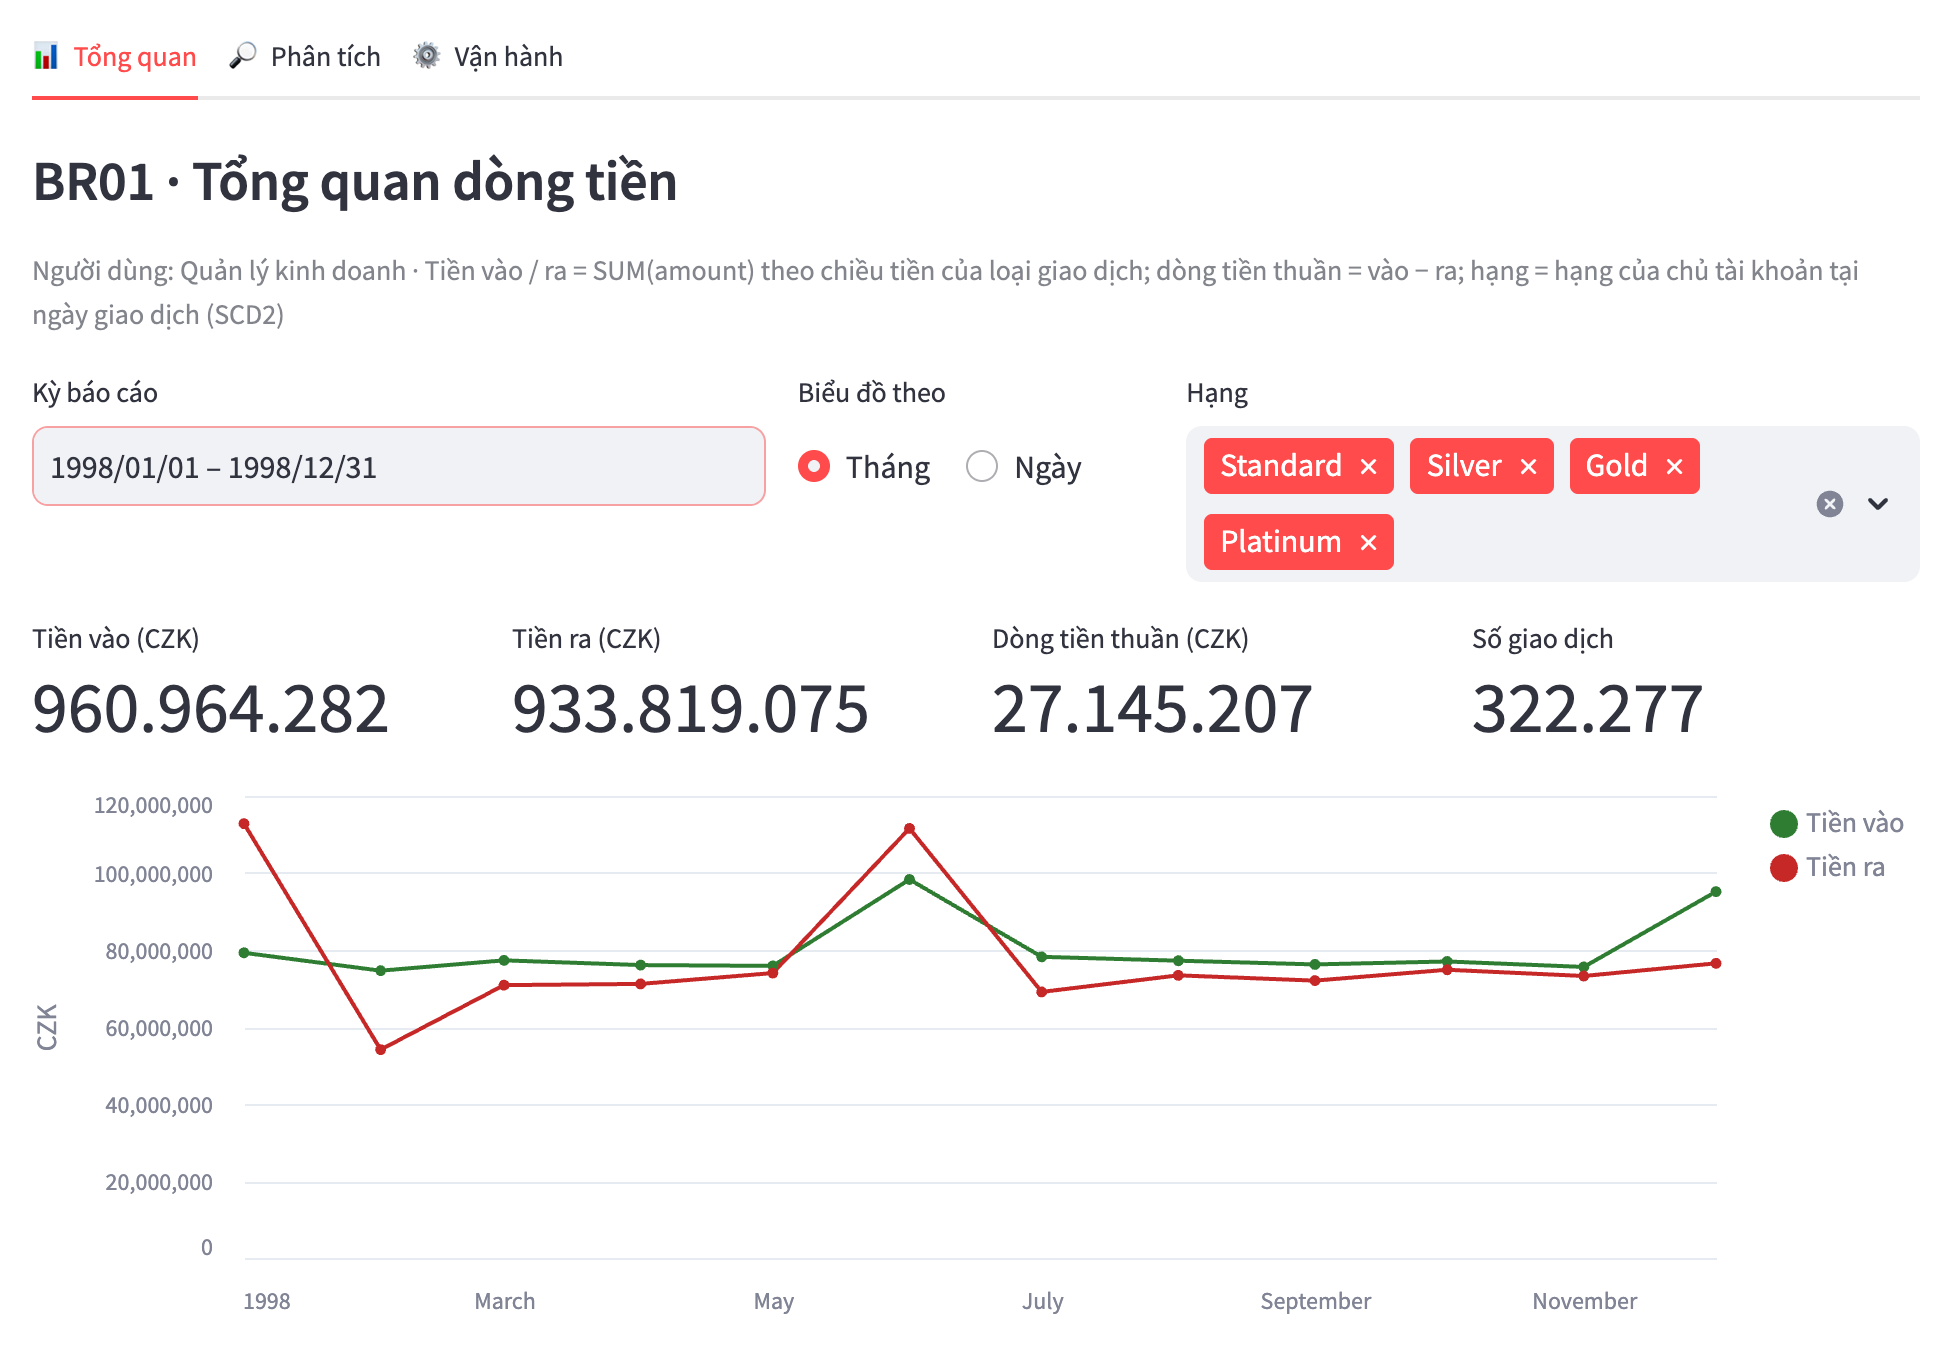
\includegraphics[width=\columnwidth]{app_overview}
\caption{Tab Tổng quan (U01, BR01): các KPI dòng tiền và biểu đồ theo tháng của năm 1998.}
\label{fig:app-overview}
\end{figure}

\begin{figure}[!t]
\centering
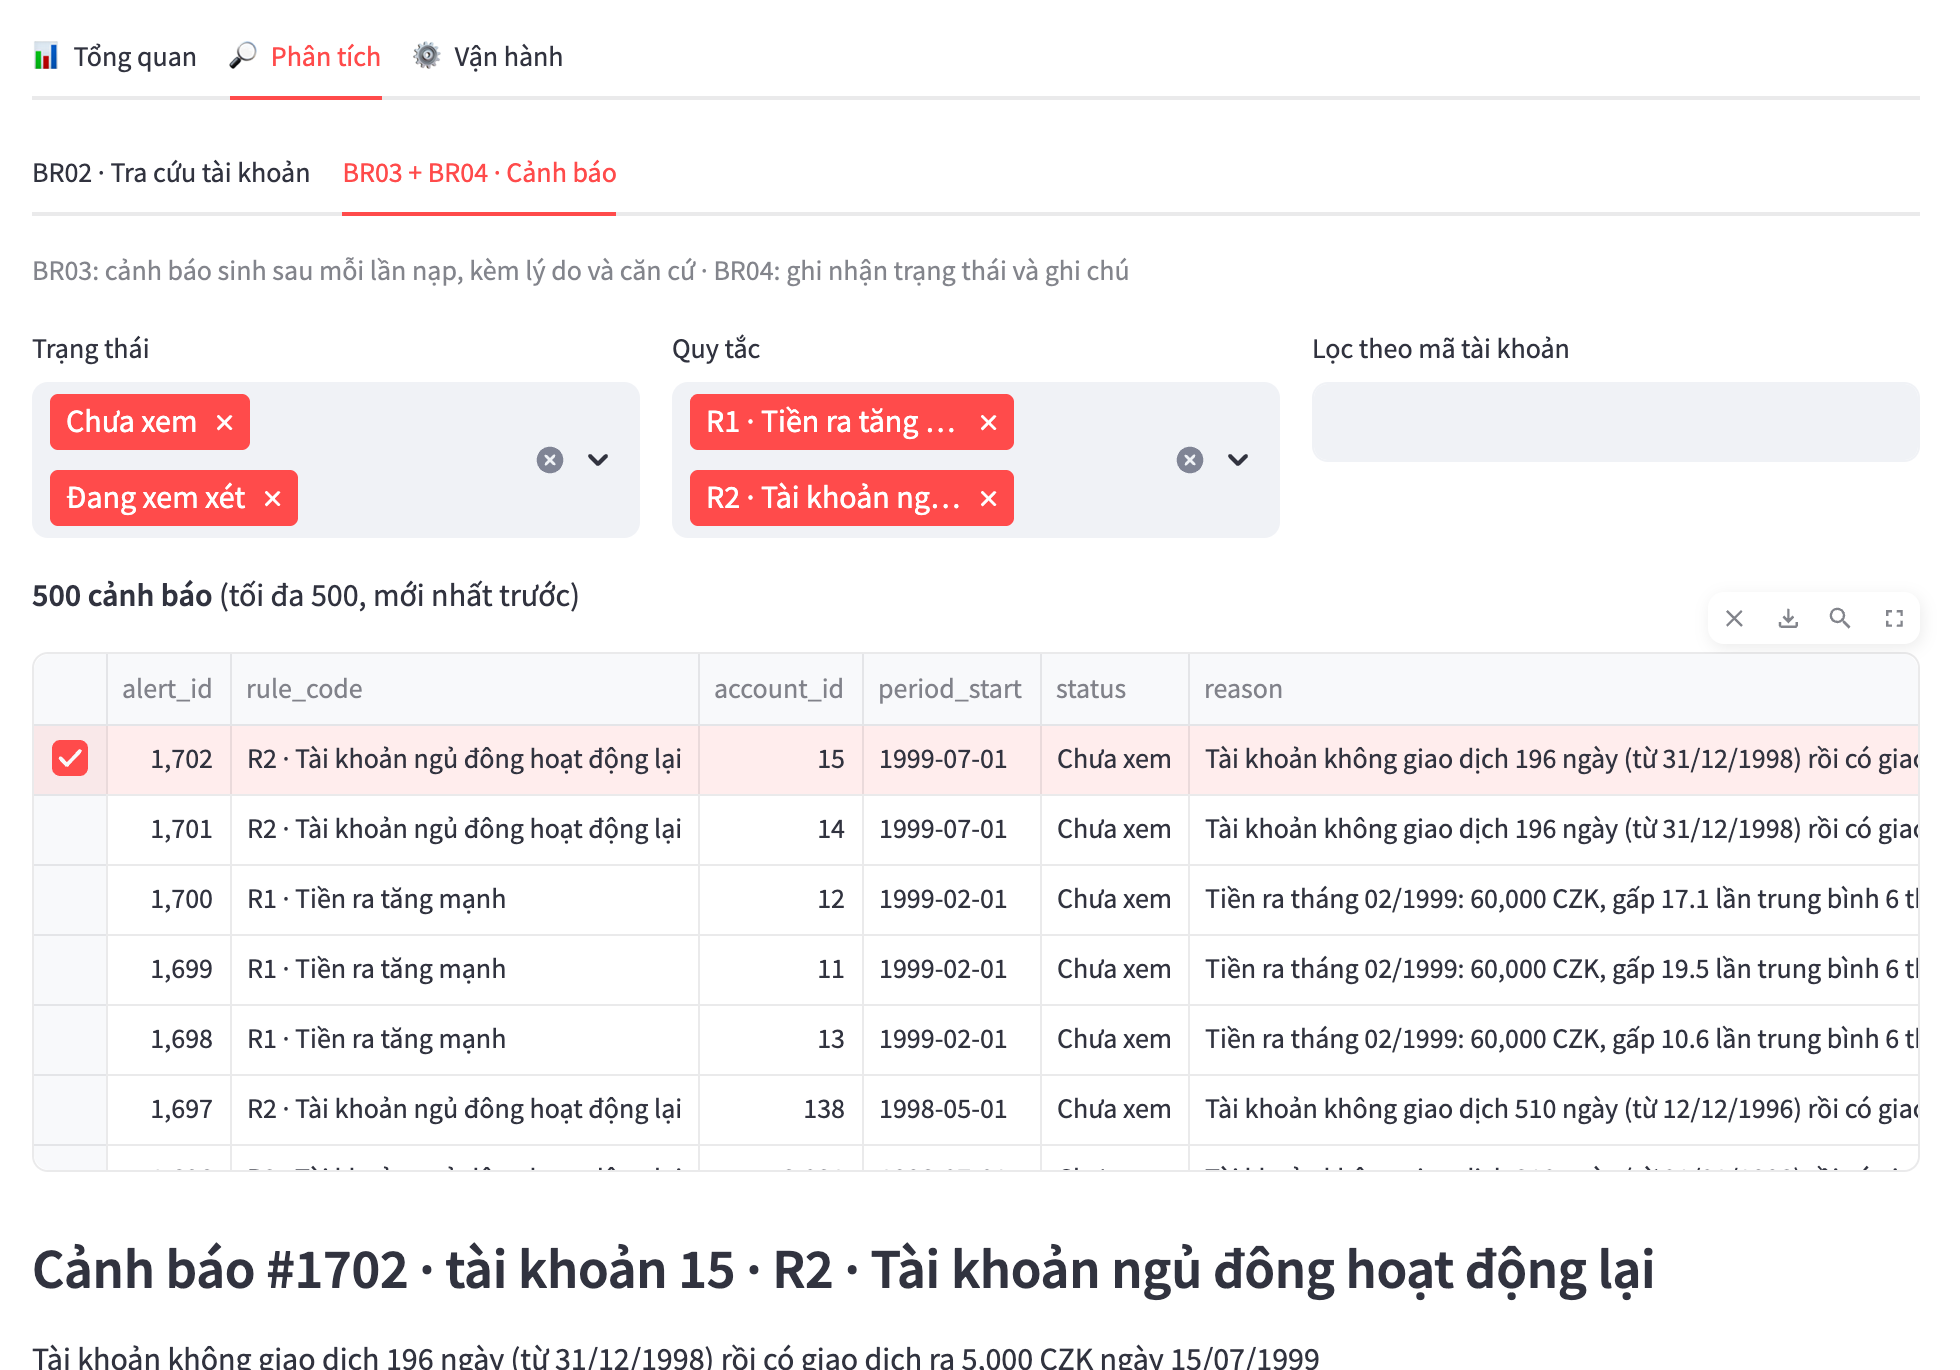
\includegraphics[width=\columnwidth]{app_alert}
\caption{Tab Phân tích (U02, BR03): danh sách cảnh báo với quy tắc, tài khoản, kỳ, trạng thái và lý do.}
\label{fig:app-alert}
\end{figure}

\subsection{Diễn giải}
Kết quả cho thấy giải pháp đề xuất đáp ứng cả ba tiêu chí. Kho dữ liệu tái tạo chính xác
nguồn, và việc tách riêng bản ghi lỗi, chạy lại lũy đẳng, cảnh báo không trùng lặp, khôi phục
và lưu giữ lịch sử hoạt động đúng như đặc tả. Cơ sở dữ liệu cột có vẻ là lựa chọn đúng cho
các truy vấn tổng hợp vốn đặc trưng cho tải của kho dữ liệu, với ưu thế tăng theo dữ liệu.
Mỗi phương án thay thế đều tốt hơn ở một điểm---PostgreSQL ở tra cứu điểm và cập nhật một
dòng, One Big Table ở các phép quét không cần nối---và kiến trúc sử dụng điểm mạnh thứ nhất ở
nơi nó quan trọng: kho vận hành.

\subsection{Các yếu tố ảnh hưởng đến tính hợp lệ}
Mọi hệ thống chạy trên cùng một máy ảo với client, và PostgreSQL dùng các thiết lập ở mức
vừa phải; phân vùng hoặc materialized view có thể thu hẹp khoảng cách của nó. Các lần chạy
``lạnh'' chỉ lạnh một phần, vì page cache của hệ điều hành không thể xóa được. Dữ liệu
$\times$10 là bản sao nhân bản và có thể nén tốt hơn dữ liệu thực. Hạng thành viên và các
kịch bản là mô phỏng, và các thao tác được đo bởi một script, không phải với người dùng thực.


%% =====================================================================
\section{Kết luận và khuyến nghị}
\label{sec:conclusion}

Kho dữ liệu Kimball trên ClickHouse, được nạp bởi một pipeline theo lô có kiểm soát và đi
kèm một kho vận hành trên PostgreSQL, đã đáp ứng cả ba tiêu chí. Về \emph{độ đúng của dữ
liệu}, cả tám kịch bản đều đạt và các số liệu dòng tiền bằng nguồn đến từng xu, với lịch sử
được lưu giữ qua các lần đổi hạng. Về \emph{hiệu năng}, ClickHouse trả lời các truy vấn tổng
hợp nhanh hơn PostgreSQL 3,3--22 lần (7--28 lần ở $\times$10) với dung lượng nhỏ hơn 8,7 lần,
star schema tránh được chi phí chỉnh sửa lên tới 1,5 triệu dòng, và kho vận hành nhanh hơn
8--70 lần và an toàn hơn trong PostgreSQL. Về \emph{hiệu quả}, mọi BR đều được trả lời với
một đến ba thao tác trong vòng nửa giây.

\textbf{Khuyến nghị.} Dùng một cơ sở dữ liệu cột cho kho dữ liệu, vì người dùng của nó chủ
yếu thực hiện tổng hợp, và một cơ sở dữ liệu quan hệ cho dữ liệu vận hành, vì dữ liệu này
được cập nhật tại chỗ và phải thực thi các ràng buộc. Trong các truy vấn tra cứu, lọc bảng
fact theo khóa của chính nó trước.

\textbf{Hạn chế và hướng phát triển.} Dữ liệu kết thúc vào năm 1998 và hạng thành viên là mô
phỏng; còn thiếu số dư cuối kỳ và kiểm soát truy cập. Hướng phát triển: kiểm soát truy cập
theo nhóm người dùng, thêm các quy trình nghiệp vụ như khoản vay, đo ở quy mô lớn hơn và trên
một cụm máy, và phát hiện bất thường dựa trên học máy, được đánh giá với cùng các kịch bản.


%% =====================================================================
\appendices

\section{Khả năng tái lập}
\label{App:Reproducibility}
Mã nguồn và các script: \url{https://github.com/quanndc/data-engineer-bank-project}.
\texttt{make up}, \texttt{make schema}, \texttt{make load-ref} và \texttt{make load-history}
xây dựng kho dữ liệu; \texttt{make scenarios} và \texttt{make scenario KB=\ldots} chạy các
kịch bản; \texttt{make evaluate} và \texttt{make bench-all} (\texttt{SCALE=10} cho
$\times$10) tái lập phần đánh giá và các benchmark, với kết quả trong
\texttt{docs/results/p2/}; \texttt{tools/ui\_walkthrough.py} đo ứng dụng.

\section{Phân công công việc}
\label{App:Work}

\todo{Xác nhận phân công với nhóm.}

\begin{table}[!h]
\centering
\caption{Phân công công việc}
\label{tab:work}
\footnotesize
\setlength{\tabcolsep}{4pt}
\begin{tabular}{L{2.6cm} L{3.4cm} L{1.6cm}}
\toprule
\textbf{Thành viên} & \textbf{Mảng kỹ thuật} & \textbf{BR} \\
\midrule
Kiet Ho Tuan Nguyen & \todo{} & \todo{} \\
Quan Minh Tran & \todo{} & \todo{} \\
Van Ngoc Huynh & \todo{} & \todo{} \\
Hai Ngoc Ho & \todo{} & \todo{} \\
\bottomrule
\end{tabular}
\end{table}


\begin{thebibliography}{99}

\bibitem{berka1999}
P.~Berka, ``Guide to the financial data set,'' in \emph{PKDD'99 Discovery Challenge},
Prague, Czech Republic, 1999. [Online]. Available:
\url{https://www.kaggle.com/datasets/marceloventura/the-berka-dataset}

\bibitem{kimball2013}
R.~Kimball and M.~Ross, \emph{The Data Warehouse Toolkit: The Definitive Guide to
Dimensional Modeling}, 3rd~ed.\hskip 1em plus 0.5em minus 0.4em\relax Indianapolis, IN,
USA: Wiley, 2013.

\bibitem{inmon2005}
W.~H. Inmon, \emph{Building the Data Warehouse}, 4th~ed.\hskip 1em plus 0.5em minus
0.4em\relax Indianapolis, IN, USA: Wiley, 2005.

\bibitem{linstedt2015}
D.~Linstedt and M.~Olschimke, \emph{Building a Scalable Data Warehouse with Data Vault
2.0}.\hskip 1em plus 0.5em minus 0.4em\relax Waltham, MA, USA: Morgan Kaufmann, 2015.

\bibitem{zaharia2016spark}
M.~Zaharia \emph{et~al.}, ``Apache Spark: A unified engine for big data processing,''
\emph{Commun. ACM}, vol.~59, no.~11, pp.~56--65, 2016.

\bibitem{schulze2024clickhouse}
R.~Schulze, T.~Schreiber, I.~Yatsishin, R.~Dahimene, and A.~Milovidov, ``ClickHouse ---
Lightning fast analytics for everyone,'' \emph{Proc. VLDB Endow.}, vol.~17, no.~12,
pp.~3731--3744, 2024.

\bibitem{stonebraker2005cstore}
M.~Stonebraker \emph{et~al.}, ``C-Store: A column-oriented DBMS,'' in \emph{Proc. VLDB},
2005, pp.~553--564.

\bibitem{abadi2008column}
D.~J. Abadi, S.~R. Madden, and N.~Hachem, ``Column-stores vs.\ row-stores: How different
are they really?'' in \emph{Proc. ACM SIGMOD}, 2008, pp.~967--980.

\bibitem{armbrust2021lakehouse}
M.~Armbrust, A.~Ghodsi, R.~Xin, and M.~Zaharia, ``Lakehouse: A new generation of open
platforms that unify data warehousing and advanced analytics,'' in \emph{Proc. CIDR}, 2021.

\bibitem{oneil2009ssb}
P.~O'Neil, E.~O'Neil, X.~Chen, and S.~Revilak, ``The Star Schema Benchmark and augmented
fact table indexing,'' in \emph{Proc. TPCTC}, LNCS vol.~5895, 2009, pp.~237--252.

\bibitem{tpch}
Transaction Processing Performance Council, ``TPC Benchmark H (Decision Support) Standard
Specification.'' [Online]. Available: \url{https://www.tpc.org/tpch/}

\bibitem{tpcds}
Transaction Processing Performance Council, ``TPC Benchmark DS Standard Specification.''
[Online]. Available: \url{https://www.tpc.org/tpcds/}

\bibitem{iso25012}
\emph{Software Engineering --- Software Product Quality Requirements and Evaluation
(SQuaRE) --- Data Quality Model}, ISO/IEC 25012:2008, 2008.

\bibitem{c4model}
S.~Brown, ``The C4 model for visualising software architecture.'' [Online]. Available:
\url{https://c4model.com}

\bibitem{streamlit}
Snowflake Inc., ``Streamlit: A faster way to build and share data apps.'' [Online].
Available: \url{https://streamlit.io}

\end{thebibliography}

\end{document}
